\chapter{Support Vector Machine}


\section{Introduction}
\begin{itemize}
    \item The cost of the $i^{th}$ item in the logistic function is
    \begin{equation} J^{(i)} = y^{(i)} \log{h^{(i)}} + (1-y^{(i)}) \log{(1-h^{(i)})} \end{equation}
    where
    \begin{equation} h^{(i)} = \frac{1}{1+e^{-\mathbf{z}}} \end{equation}
    
    \item Plot the cost functions as $y=1$ and $y=0$. SVM use the approximated costs named as $L_1$ and $L_0$.
    \begin{figure}[!htbp]
        \begin{minipage}[t]{0.5\textwidth}
            \centering
            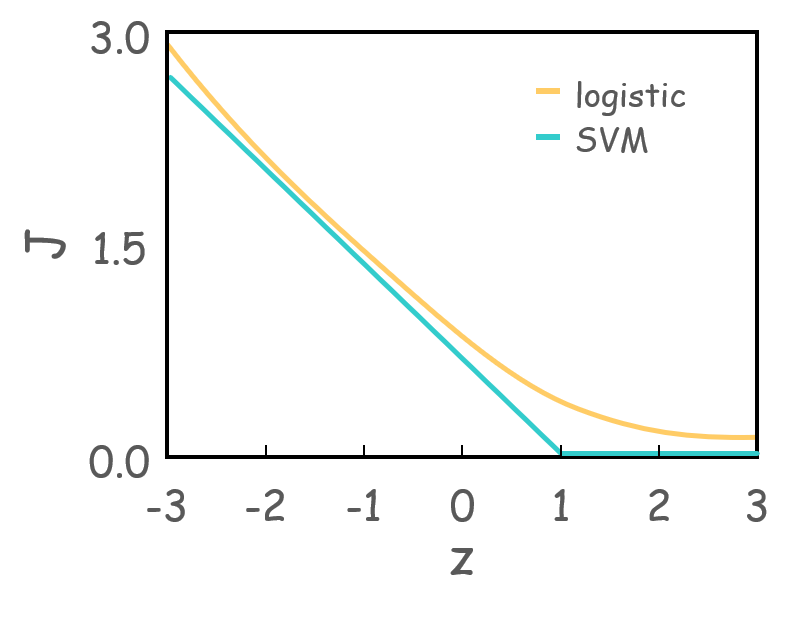
\includegraphics[width=2.0in]{./images/supportVectorMachineY1.png}
            \caption{The cost function as $y=1$}
        \end{minipage}
        \begin{minipage}[t]{0.45\textwidth}
            \centering
            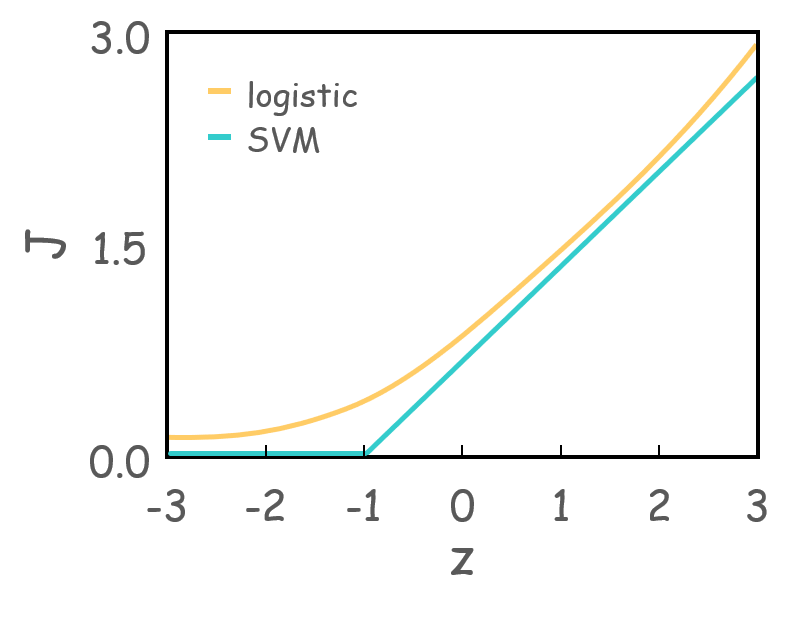
\includegraphics[width=2.0in]{./images/supportVectorMachineY0.png}
            \caption{The cost function as $y=0$}
        \end{minipage}
    \end{figure}
\end{itemize}


\section{The optimization of the cost function}
\begin{itemize}
\item The object of the optimization is
\begin{equation} \min_\theta \frac{1}{m} \sum_{i=0}^{m} \left[y^{(i)} L_1(z^{(i)}) + (1-y^{(i)}) L_0(z^{(i)}) \right] + \frac{\lambda}{2m} \sum_{j=1}^{n} \theta_j^2 \end{equation}
As $z^{(i)} = \mathbf{x}^{(i)}\theta$. When $z^{(i)} \geq 1$ or $z^{(i)} \leq -1$, the first term in the cost is zero, only the regularization term will remain.
As a result, the total cost would only remain
\begin{equation} \min_\theta \sum_{j=1}^{n} \theta_j^2 \end{equation}

And that is to say
\begin{equation}
    \min_\theta \sum_{j=1}^{n} \theta_j^2 = \min_\theta{\left\|\theta\right\|}^2 = \min_\theta{\left\|\theta\right\|}
\end{equation}

\item Observe $\mathbf{x}^{(i)}\theta$. This can be seen as an inner product of two vectors $\theta$ and $\mathbf{x}^{(i)}$. Where
\begin{equation} \theta = \left[{\begin{matrix} \theta_0 & \theta_1 & \dots & \theta_n \end{matrix}}\right]^T \end{equation}
\begin{equation} \mathbf{x}^{(i)} = \left[{\begin{matrix} x_0^{(i)} & x_1^{(i)} & \dots & x_n^{(i)} \end{matrix}}\right] \end{equation}
Assum the angle between $\theta$ and $\mathbf{x}^{(i)}$ is $\varphi^{(i)}$. That is to say
\begin{equation}
    \begin{aligned}
        \mathbf{x}^{(i)}\theta &= \left\| \mathbf{x}^{(i)} \right\| \left\| \theta \right\| \cos\varphi^{(i)} \\
                               &= p^{(i)} \left\| \theta \right\| \sign\varphi^{(i)}
    \end{aligned}
\end{equation}
Where $p^{(i)}$ is the projection of $\mathbf{x}^{(i)}$ onto $\theta$

\item Now the question is how to minimize the cost function. In cases of margin classification. The following must be satisfied
\begin{equation}
    \left\{ \begin{aligned}
        \mathbf{x}^{(i)}\theta &= \left\| \theta \right\| p^{(i)} &\geq 1 & \text{, for } x^{(i)}\\
        \mathbf{x}^{(j)}\theta &= -\left\| \theta \right\| p^{(j)} &\leq 1 & \text{, for } x^{(j)}\\
    \end{aligned} \right.
\end{equation}
It's obvious to see that as $p^{(i)}$ and $p^{(j)}$ get larger, a smaller $\| \theta \|$ would be needed to satisfy the inequality.
That implies \emph{when $\theta$ in the direcction to make a maximized margin, then the total cost would be minimized.}
\begin{figure}[!htbp]
    \centering
    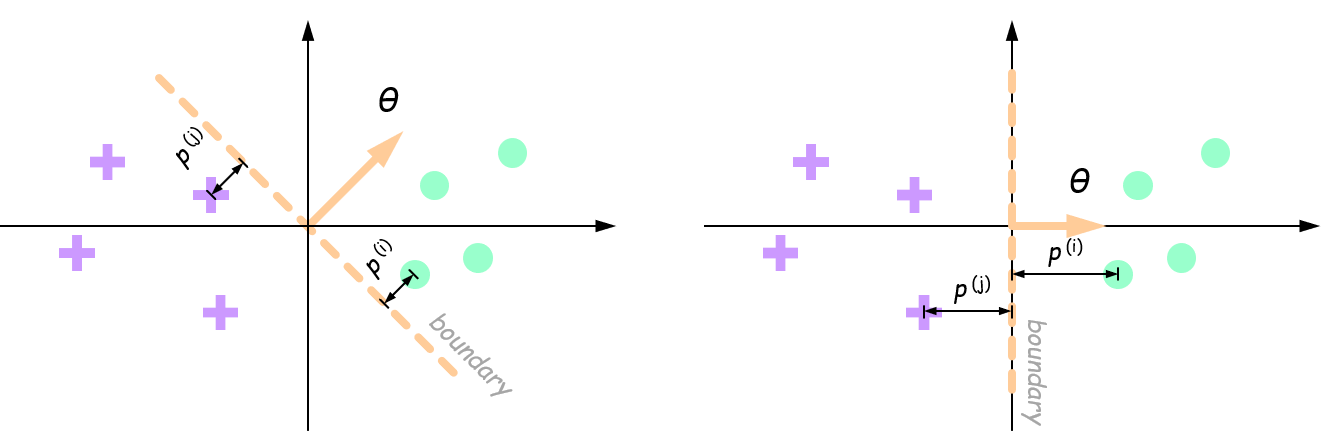
\includegraphics[width=4.8in]{./images/marginClassification.png}
    \caption{Margin classification with different $\theta$}
\end{figure}
\end{itemize}


\section{Gaussian kernel}
\begin{itemize}
\item Gaussian kernel can make prediction of input data with a non-linear decision boundary. Given $m$ data, then choose these data as landmarks.
\begin{equation}
    \begin{array}{cccc}
        l^{(1)} = x^{(1)} & l^{(2)} = x^{(2)} & \dots & l^{(m)} = x^{(m)}
    \end{array}
\end{equation}

\item Define the \emph{similarity function}
\begin{equation}
    \begin{aligned}
        f_{j}^{(i)} &= f(x^{(i)}, l^{(j)}) \\
        &= \exp\left({-\frac{\left\|x^{(i)} - l^{(j)}\right\|^2}{2\sigma^2}}\right)
    \end{aligned}
\end{equation}
Then the values of the similarity fuctions would be
\begin{equation}
    f_{j}^{(i)} \approx
    \left\{\begin{aligned}
        1 &\text{, for } x^{(i)} \approx l^{(j)}\\
        0 &\text{, for } x^{(i)} \neq l^{(j)}\\
    \end{aligned}\right.
\end{equation}
\begin{figure}[!htbp]
    \centering
    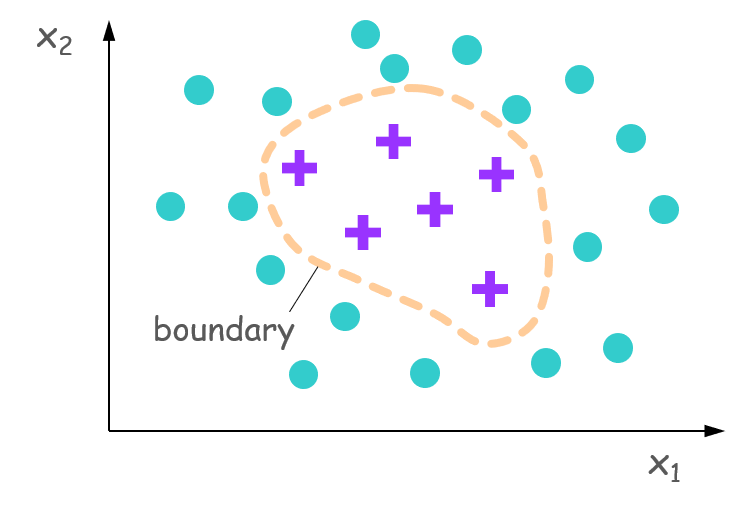
\includegraphics[width=2.8in]{./images/nonlinearDecisionBoundary.png}
    \caption{Non-linear decision boundary}
\end{figure}

\item For each similarity functions, its distribution looks like
\begin{figure}[!htbp]
    \centering
    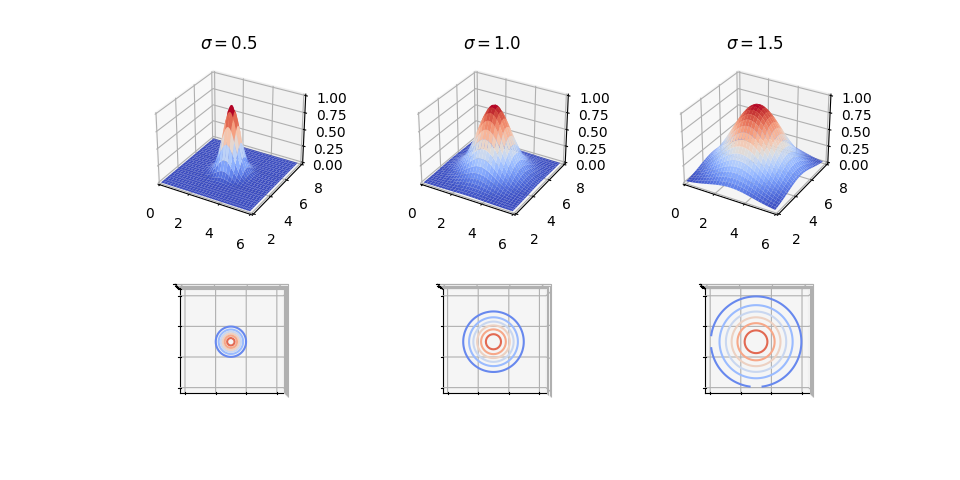
\includegraphics[width=7.0in]{./images/gaussianKernel.png}
    \caption{Gaussian kernel functions}
\end{figure}

\item For training example $x^{(i)}$, all of its similarity would be
\begin{equation}
    \mathbf{f}^{(i)} = \left[\begin{matrix}
        f_0^{(i)} \\ f_1^{(i)} \\ f_2^{(i)} \\ \vdots \\ f_m^{(i)}
    \end{matrix}\right] = 
    \left[\begin{matrix}
        1 \\ f(x^{(i)}, l^{(1)}) \\ f(x^{(i)}, l^{(2)}) \\ \vdots \\ f(x^{(i)}, l^{(m)})
    \end{matrix}\right]
\end{equation}
The $i^{th}$ item in the array is
\begin{equation}
    f_i^{(i)} = f(x^{(i)}, l^{(i)}) = 1
\end{equation}

\item So, how does Gaussian kernel work? Assume
\begin{equation}
    z^{(i)} = \theta^T\mathbf{f}^{(i)}
\end{equation}

Put $z^{(i)}$ to the sigmoid function.
\begin{equation}
    g^{(i)} = \frac{1}{1+e^{-z^{(i)}}}
\end{equation}

Then the decision boundary would be
\begin{equation}
    \begin{split}
        z^{(i)} = \theta^T \mathbf{f}^{(i)} & \geq 0 \Rightarrow g^{(i)} \geq 0.5 \Rightarrow y^{(i)} = 1\\
        z^{(i)} = \theta^T \mathbf{f}^{(i)} & <    0 \Rightarrow g^{(i)} <    0.5 \Rightarrow y^{(i)} = 0
    \end{split}
\end{equation}

Then the total cost become
\begin{equation}
    \min_\theta \frac{1}{m} \sum_{i=0}^{m} \left[{y^{(i)} L_1(z^{(i)}) + (1-y^{(i)}) L_0(z^{(i)}) }\right] + \frac{\lambda}{2m} \sum_{j=1}^{m} \theta_j^2
\end{equation}
\end{itemize}

